\section{}
% A 40 mm diameter bar ABC is composed of an aluminum part AB and a steel part BC as shown
% in Fig. 3. After axial force P is applied, a strain gage attached to the steel measures normal strain
% at the longitudinal direction as εs = 600 μ. Determine,
% (a) the magnitude of the applied force P .
% (b) the total elongation of the bar if each material behaves elastically. Take Ealuminum = 70 GPa
% and Esteel = 210 GPa.
% Figure 3: A composite steel rod
% 4

A 40 mm diameter bar $ABC$ is composed of an aluminum part $AB$ and a steel part $BC$ as shown in Fig. \ref{fig:fig3}. 
After axial force $P$ is applied, a strain gage attached to the steel measures normal strain at the longitudinal direction 
as $\epsilon_s = 600 \mu$. Determine,
\begin{enumerate}[label=(\alph*)]
    \item the magnitude of the applied force $P$.
    \item the total elongation of the bar if each material behaves elastically. Take $E_{\text{aluminum}} = \qty{70}{\giga\pascal}$ 
    and $E_{\text{steel}} = \qty{210}{\giga\pascal}$.  
\end{enumerate}

\begin{figure}[h]
    \centering
    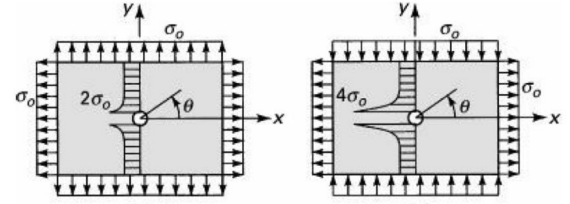
\includegraphics[width=0.3\linewidth]{Questions/Figures/Q4ProblemDiagram.png}
    \caption{A composite steel rod}
    \label{fig:fig3}
\end{figure}

\subsection{}
By Hooke's Law, the strain in the steel part is given by:
% \begin{align*}
%     \sigma_s &= E_{steel}\epsilon_s \\
%     \frac{P}{A_{steel}} &= E_{steel}\epsilon_s \\
%     P &= E_{steel}A_{steel}\epsilon_s \\
%     &= 210 \times \frac{\pi}{4} \times (40)^2 \times 600 \times 10^{-6} \\
%     &= \boxed{\qty{158}{\kilo\newton}}
% \end{align*}
\begin{align*}
    \sigma_s &= E_{\text{steel}}\epsilon_s \\
    \frac{P}{A_{\text{steel}}} &= E_{\text{steel}}\epsilon_s \\
    P &= E_{\text{steel}}A_{\text{steel}}\epsilon_s \\
    &= 210 \times \frac{\pi}{4} \times (40)^2 \times 600 \times 10^{-6} \\
    &= \boxed{\qty{158}{\kilo\newton}}
\end{align*}

\subsection{}
The total elongation of the bar is given by the addition of the elongation of the aluminum and steel parts. First
we find the strain in the aluminum part:
\begin{align*}
    \epsilon_{\text{aluminum}} &= \frac{P}{A_{\text{aluminum}}E_{\text{aluminum}}} \\
    &= \frac{158}{\frac{\pi}{4}(40)^2(70)} \\
    &= \qty{1.796e-3}{} \\
\end{align*}

Next, 
\begin{align*}
    \Delta L &= \epsilon_{\text{aluminum}}L_{\text{aluminum}} + \epsilon_{\text{steel}}L_{\text{steel}} \\
    &= \qty{1.796e-3}{}(0.5\times 10^3) + \qty{600e-6}{}(1.5\times 10^3) \\
    &= \boxed{\qty{1.80}{\milli\meter}}
\end{align*}